
%% bare_jrnl.tex
%% V1.4
%% 2012/12/27
%% by Michael Shell
%% see http://www.michaelshell.org/
%% for current contact information.
%%
%% This is a skeleton file demonstrating the use of IEEEtran.cls
%% (requires IEEEtran.cls version 1.8 or later) with an IEEE journal paper.
%%
%% Support sites:
%% http://www.michaelshell.org/tex/ieeetran/
%% http://www.ctan.org/tex-archive/macros/latex/contrib/IEEEtran/
%% and
%% http://www.ieee.org/



% *** Authors should verify (and, if needed, correct) their LaTeX system  ***
% *** with the testflow diagnostic prior to trusting their LaTeX platform ***
% *** with production work. IEEE's font choices can trigger bugs that do  ***
% *** not appear when using other class files.                            ***
% The testflow support page is at:
% http://www.michaelshell.org/tex/testflow/


%%*************************************************************************
%% Legal Notice:
%% This code is offered as-is without any warranty either expressed or
%% implied; without even the implied warranty of MERCHANTABILITY or
%% FITNESS FOR A PARTICULAR PURPOSE! 
%% User assumes all risk.
%% In no event shall IEEE or any contributor to this code be liable for
%% any damages or losses, including, but not limited to, incidental,
%% consequential, or any other damages, resulting from the use or misuse
%% of any information contained here.
%%
%% All comments are the opinions of their respective authors and are not
%% necessarily endorsed by the IEEE.
%%
%% This work is distributed under the LaTeX Project Public License (LPPL)
%% ( http://www.latex-project.org/ ) version 1.3, and may be freely used,
%% distributed and modified. A copy of the LPPL, version 1.3, is included
%% in the base LaTeX documentation of all distributions of LaTeX released
%% 2003/12/01 or later.
%% Retain all contribution notices and credits.
%% ** Modified files should be clearly indicated as such, including  **
%% ** renaming them and changing author support contact information. **
%%
%% File list of work: IEEEtran.cls, IEEEtran_HOWTO.pdf, bare_adv.tex,
%%                    bare_conf.tex, bare_jrnl.tex, bare_jrnl_compsoc.tex,
%%                    bare_jrnl_transmag.tex
%%*************************************************************************

% Note that the a4paper option is mainly intended so that authors in
% countries using A4 can easily print to A4 and see how their papers will
% look in print - the typesetting of the document will not typically be
% affected with changes in paper size (but the bottom and side margins will).
% Use the testflow package mentioned above to verify correct handling of
% both paper sizes by the user's LaTeX system.
%
% Also note that the "draftcls" or "draftclsnofoot", not "draft", option
% should be used if it is desired that the figures are to be displayed in
% draft mode.
%
\documentclass[journal]{IEEEtran}
%
% If IEEEtran.cls has not been installed into the LaTeX system files,
% manually specify the path to it like:
% \documentclass[journal]{../sty/IEEEtran}





% Some very useful LaTeX packages include:
% (uncomment the ones you want to load)


% *** MISC UTILITY PACKAGES ***
%
%\usepackage{ifpdf}
% Heiko Oberdiek's ifpdf.sty is very useful if you need conditional
% compilation based on whether the output is pdf or dvi.
% usage:
% \ifpdf
%   % pdf code
% \else
%   % dvi code
% \fi
% The latest version of ifpdf.sty can be obtained from:
% http://www.ctan.org/tex-archive/macros/latex/contrib/oberdiek/
% Also, note that IEEEtran.cls V1.7 and later provides a builtin
% \ifCLASSINFOpdf conditional that works the same way.
% When switching from latex to pdflatex and vice-versa, the compiler may
% have to be run twice to clear warning/error messages.






% *** CITATION PACKAGES ***
%
%\usepackage{cite}
% cite.sty was written by Donald Arseneau
% V1.6 and later of IEEEtran pre-defines the format of the cite.sty package
% \cite{} output to follow that of IEEE. Loading the cite package will
% result in citation numbers being automatically sorted and properly
% "compressed/ranged". e.g., [1], [9], [2], [7], [5], [6] without using
% cite.sty will become [1], [2], [5]--[7], [9] using cite.sty. cite.sty's
% \cite will automatically add leading space, if needed. Use cite.sty's
% noadjust option (cite.sty V3.8 and later) if you want to turn this off
% such as if a citation ever needs to be enclosed in parenthesis.
% cite.sty is already installed on most LaTeX systems. Be sure and use
% version 4.0 (2003-05-27) and later if using hyperref.sty. cite.sty does
% not currently provide for hyperlinked citations.
% The latest version can be obtained at:
% http://www.ctan.org/tex-archive/macros/latex/contrib/cite/
% The documentation is contained in the cite.sty file itself.






% *** GRAPHICS RELATED PACKAGES ***
%
\ifCLASSINFOpdf
   \usepackage[pdftex]{graphicx}
  % declare the path(s) where your graphic files are
  % \graphicspath{{../pdf/}{../jpeg/}}
  % and their extensions so you won't have to specify these with
  % every instance of \includegraphics
  % \DeclareGraphicsExtensions{.pdf,.jpeg,.png}
\else
  % or other class option (dvipsone, dvipdf, if not using dvips). graphicx
  % will default to the driver specified in the system graphics.cfg if no
  % driver is specified.
  % \usepackage[dvips]{graphicx}
  % declare the path(s) where your graphic files are
  % \graphicspath{{../eps/}}
  % and their extensions so you won't have to specify these with
  % every instance of \includegraphics
  % \DeclareGraphicsExtensions{.eps}
\fi
% graphicx was written by David Carlisle and Sebastian Rahtz. It is
% required if you want graphics, photos, etc. graphicx.sty is already
% installed on most LaTeX systems. The latest version and documentation
% can be obtained at: 
% http://www.ctan.org/tex-archive/macros/latex/required/graphics/
% Another good source of documentation is "Using Imported Graphics in
% LaTeX2e" by Keith Reckdahl which can be found at:
% http://www.ctan.org/tex-archive/info/epslatex/
%
% latex, and pdflatex in dvi mode, support graphics in encapsulated
% postscript (.eps) format. pdflatex in pdf mode supports graphics
% in .pdf, .jpeg, .png and .mps (metapost) formats. Users should ensure
% that all non-photo figures use a vector format (.eps, .pdf, .mps) and
% not a bitmapped formats (.jpeg, .png). IEEE frowns on bitmapped formats
% which can result in "jaggedy"/blurry rendering of lines and letters as
% well as large increases in file sizes.
%
% You can find documentation about the pdfTeX application at:
% http://www.tug.org/applications/pdftex





% *** MATH PACKAGES ***
%
%\usepackage[cmex10]{amsmath}
% A popular package from the American Mathematical Society that provides
% many useful and powerful commands for dealing with mathematics. If using
% it, be sure to load this package with the cmex10 option to ensure that
% only type 1 fonts will utilized at all point sizes. Without this option,
% it is possible that some math symbols, particularly those within
% footnotes, will be rendered in bitmap form which will result in a
% document that can not be IEEE Xplore compliant!
%
% Also, note that the amsmath package sets \interdisplaylinepenalty to 10000
% thus preventing page breaks from occurring within multiline equations. Use:
%\interdisplaylinepenalty=2500
% after loading amsmath to restore such page breaks as IEEEtran.cls normally
% does. amsmath.sty is already installed on most LaTeX systems. The latest
% version and documentation can be obtained at:
% http://www.ctan.org/tex-archive/macros/latex/required/amslatex/math/





% *** SPECIALIZED LIST PACKAGES ***
%
%\usepackage{algorithmic}
% algorithmic.sty was written by Peter Williams and Rogerio Brito.
% This package provides an algorithmic environment fo describing algorithms.
% You can use the algorithmic environment in-text or within a figure
% environment to provide for a floating algorithm. Do NOT use the algorithm
% floating environment provided by algorithm.sty (by the same authors) or
% algorithm2e.sty (by Christophe Fiorio) as IEEE does not use dedicated
% algorithm float types and packages that provide these will not provide
% correct IEEE style captions. The latest version and documentation of
% algorithmic.sty can be obtained at:
% http://www.ctan.org/tex-archive/macros/latex/contrib/algorithms/
% There is also a support site at:
% http://algorithms.berlios.de/index.html
% Also of interest may be the (relatively newer and more customizable)
% algorithmicx.sty package by Szasz Janos:
% http://www.ctan.org/tex-archive/macros/latex/contrib/algorithmicx/




% *** ALIGNMENT PACKAGES ***
%
%\usepackage{array}
% Frank Mittelbach's and David Carlisle's array.sty patches and improves
% the standard LaTeX2e array and tabular environments to provide better
% appearance and additional user controls. As the default LaTeX2e table
% generation code is lacking to the point of almost being broken with
% respect to the quality of the end results, all users are strongly
% advised to use an enhanced (at the very least that provided by array.sty)
% set of table tools. array.sty is already installed on most systems. The
% latest version and documentation can be obtained at:
% http://www.ctan.org/tex-archive/macros/latex/required/tools/


% IEEEtran contains the IEEEeqnarray family of commands that can be used to
% generate multiline equations as well as matrices, tables, etc., of high
% quality.




% *** SUBFIGURE PACKAGES ***
\ifCLASSOPTIONcompsoc
  \usepackage[caption=false,font=normalsize,labelfont=sf,textfont=sf]{subfig}
\else
  \usepackage[caption=false,font=footnotesize]{subfig}
\fi
% subfig.sty, written by Steven Douglas Cochran, is the modern replacement
% for subfigure.sty, the latter of which is no longer maintained and is
% incompatible with some LaTeX packages including fixltx2e. However,
% subfig.sty requires and automatically loads Axel Sommerfeldt's caption.sty
% which will override IEEEtran.cls' handling of captions and this will result
% in non-IEEE style figure/table captions. To prevent this problem, be sure
% and invoke subfig.sty's "caption=false" package option (available since
% subfig.sty version 1.3, 2005/06/28) as this is will preserve IEEEtran.cls
% handling of captions.
% Note that the Computer Society format requires a larger sans serif font
% than the serif footnote size font used in traditional IEEE formatting
% and thus the need to invoke different subfig.sty package options depending
% on whether compsoc mode has been enabled.
%
% The latest version and documentation of subfig.sty can be obtained at:
% http://www.ctan.org/tex-archive/macros/latex/contrib/subfig/




% *** FLOAT PACKAGES ***
%
%\usepackage{fixltx2e}
% fixltx2e, the successor to the earlier fix2col.sty, was written by
% Frank Mittelbach and David Carlisle. This package corrects a few problems
% in the LaTeX2e kernel, the most notable of which is that in current
% LaTeX2e releases, the ordering of single and double column floats is not
% guaranteed to be preserved. Thus, an unpatched LaTeX2e can allow a
% single column figure to be placed prior to an earlier double column
% figure. The latest version and documentation can be found at:
% http://www.ctan.org/tex-archive/macros/latex/base/


%\usepackage{stfloats}
% stfloats.sty was written by Sigitas Tolusis. This package gives LaTeX2e
% the ability to do double column floats at the bottom of the page as well
% as the top. (e.g., "\begin{figure*}[!b]" is not normally possible in
% LaTeX2e). It also provides a command:
%\fnbelowfloat
% to enable the placement of footnotes below bottom floats (the standard
% LaTeX2e kernel puts them above bottom floats). This is an invasive package
% which rewrites many portions of the LaTeX2e float routines. It may not work
% with other packages that modify the LaTeX2e float routines. The latest
% version and documentation can be obtained at:
% http://www.ctan.org/tex-archive/macros/latex/contrib/sttools/
% Do not use the stfloats baselinefloat ability as IEEE does not allow
% \baselineskip to stretch. Authors submitting work to the IEEE should note
% that IEEE rarely uses double column equations and that authors should try
% to avoid such use. Do not be tempted to use the cuted.sty or midfloat.sty
% packages (also by Sigitas Tolusis) as IEEE does not format its papers in
% such ways.
% Do not attempt to use stfloats with fixltx2e as they are incompatible.
% Instead, use Morten Hogholm'a dblfloatfix which combines the features
% of both fixltx2e and stfloats:
%
% \usepackage{dblfloatfix}
% The latest version can be found at:
% http://www.ctan.org/tex-archive/macros/latex/contrib/dblfloatfix/




%\ifCLASSOPTIONcaptionsoff
%  \usepackage[nomarkers]{endfloat}
% \let\MYoriglatexcaption\caption
% \renewcommand{\caption}[2][\relax]{\MYoriglatexcaption[#2]{#2}}
%\fi
% endfloat.sty was written by James Darrell McCauley, Jeff Goldberg and 
% Axel Sommerfeldt. This package may be useful when used in conjunction with 
% IEEEtran.cls'  captionsoff option. Some IEEE journals/societies require that
% submissions have lists of figures/tables at the end of the paper and that
% figures/tables without any captions are placed on a page by themselves at
% the end of the document. If needed, the draftcls IEEEtran class option or
% \CLASSINPUTbaselinestretch interface can be used to increase the line
% spacing as well. Be sure and use the nomarkers option of endfloat to
% prevent endfloat from "marking" where the figures would have been placed
% in the text. The two hack lines of code above are a slight modification of
% that suggested by in the endfloat docs (section 8.4.1) to ensure that
% the full captions always appear in the list of figures/tables - even if
% the user used the short optional argument of \caption[]{}.
% IEEE papers do not typically make use of \caption[]'s optional argument,
% so this should not be an issue. A similar trick can be used to disable
% captions of packages such as subfig.sty that lack options to turn off
% the subcaptions:
% For subfig.sty:
% \let\MYorigsubfloat\subfloat
% \renewcommand{\subfloat}[2][\relax]{\MYorigsubfloat[]{#2}}
% However, the above trick will not work if both optional arguments of
% the \subfloat command are used. Furthermore, there needs to be a
% description of each subfigure *somewhere* and endfloat does not add
% subfigure captions to its list of figures. Thus, the best approach is to
% avoid the use of subfigure captions (many IEEE journals avoid them anyway)
% and instead reference/explain all the subfigures within the main caption.
% The latest version of endfloat.sty and its documentation can obtained at:
% http://www.ctan.org/tex-archive/macros/latex/contrib/endfloat/
%
% The IEEEtran \ifCLASSOPTIONcaptionsoff conditional can also be used
% later in the document, say, to conditionally put the References on a 
% page by themselves.




% *** PDF, URL AND HYPERLINK PACKAGES ***
%
\usepackage{url}
% url.sty was written by Donald Arseneau. It provides better support for
% handling and breaking URLs. url.sty is already installed on most LaTeX
% systems. The latest version and documentation can be obtained at:
% http://www.ctan.org/tex-archive/macros/latex/contrib/url/
% Basically, \url{my_url_here}.




% *** Do not adjust lengths that control margins, column widths, etc. ***
% *** Do not use packages that alter fonts (such as pslatex).         ***
% There should be no need to do such things with IEEEtran.cls V1.6 and later.
% (Unless specifically asked to do so by the journal or conference you plan
% to submit to, of course. )


% correct bad hyphenation here
\hyphenation{op-tical net-works semi-conduc-tor}

% OWN PACKAGES
\usepackage[english]{babel} % For fixing the tilde problem https://bugs.launchpad.net/ubuntu/+source/texinfo/+bug/526974
\usepackage{paralist} % compact item

% For commenting
\usepackage{color}
\newcommand\newnotecommand[3]{%
  \newcommand#1[1]{{\color{#3}\footnote{{\color{#3}#2:} ##1}}}}
\newnotecommand\joni{Joni}{red}
\newnotecommand\anders{Anders}{blue}
\newnotecommand\norbert{Norbert}{green}


\begin{document}
%
% paper title
% can use linebreaks \\ within to get better formatting as desired
% Do not put math or special symbols in the title.
\title{Bare Demo of IEEEtran.cls for Journals}
\title{A comparison of local feature detectors and descriptors by intra-class repeatability and matching}
\title{A Comparison of Feature Detectors and Descriptors for Visual Object Class Matching}

%
%
% author names and IEEE memberships
% note positions of commas and nonbreaking spaces ( ~ ) LaTeX will not break
% a structure at a ~ so this keeps an author's name from being broken across
% two lines.
% use \thanks{} to gain access to the first footnote area
% a separate \thanks must be used for each paragraph as LaTeX2e's \thanks
% was not built to handle multiple paragraphs
%

\author{Jukka~Lankinen,
Anders~Glent~Buch,
Ville~Kangas,
Joni-Kristian~K\"am\"ar\"ainen,
Norbert~Kr\"uger%
%Michael~Shell,~\IEEEmembership{Member,~IEEE,}
%        John~Doe,~\IEEEmembership{Fellow,~OSA,}
%        and~Jane~Doe,~\IEEEmembership{Life~Fellow,~IEEE}% <-this % stops a space
%\thanks{M. Shell is with the Department
%of Electrical and Computer Engineering, Georgia Institute of Technology, Atlanta,
%GA, 30332 USA e-mail: (see http://www.michaelshell.org/contact.html).}% <-this % stops a space
%\thanks{J. Doe and J. Doe are with Anonymous University.}% <-this % stops a space
%\thanks{Manuscript received April 19, 2005; revised December 27, 2012.}}
\thanks{J. Lankinen and V. Kangas are with the Department of Mathematics and Physics,
Lappeenranta University of Technology, Finland e-mail: (see http://www2.it.lut.fi/mvpr/).}%
\thanks{A.G. Buch and N. Kr\"uger are with M{\ae}rsk McKinney M{\o}ller Institute, University of Southern Denmark, Denmark}% <-this % stops a space
\thanks{J.-K. Kamarainen is with the Department of Signal Processing, Tampere University of Technology, Finland}}

% note the % following the last \IEEEmembership and also \thanks - 
% these prevent an unwanted space from occurring between the last author name
% and the end of the author line. i.e., if you had this:
% 
% \author{....lastname \thanks{...} \thanks{...} }
%                     ^------------^------------^----Do not want these spaces!
%
% a space would be appended to the last name and could cause every name on that
% line to be shifted left slightly. This is one of those "LaTeX things". For
% instance, "\textbf{A} \textbf{B}" will typeset as "A B" not "AB". To get
% "AB" then you have to do: "\textbf{A}\textbf{B}"
% \thanks is no different in this regard, so shield the last } of each \thanks
% that ends a line with a % and do not let a space in before the next \thanks.
% Spaces after \IEEEmembership other than the last one are OK (and needed) as
% you are supposed to have spaces between the names. For what it is worth,
% this is a minor point as most people would not even notice if the said evil
% space somehow managed to creep in.



% The paper headers
\markboth{IEEE Transactions on Image Processing,~Vol.~1, No.~1, December~2015}%
{Lankinen \MakeLowercase{\textit{et al.}}: Our Final Submission Title}
% The only time the second header will appear is for the odd numbered pages
% after the title page when using the twoside option.
% 
% *** Note that you probably will NOT want to include the author's ***
% *** name in the headers of peer review papers.                   ***
% You can use \ifCLASSOPTIONpeerreview for conditional compilation here if
% you desire.




% If you want to put a publisher's ID mark on the page you can do it like
% this:
%\IEEEpubid{0000--0000/00\$00.00~\copyright~2012 IEEE}
% Remember, if you use this you must call \IEEEpubidadjcol in the second
% column for its text to clear the IEEEpubid mark.



% use for special paper notices
%\IEEEspecialpapernotice{(Invited Paper)}




% make the title area
\maketitle

% As a general rule, do not put math, special symbols or citations
% in the abstract or keywords.
\begin{abstract}
Solid protocols to benchmark local
feature detectors and descriptors were introduced in Mikolajczyk
et al.~2005~\cite{MikTuySch:2005} and Mikolajczyk and
Schmid~2005~\cite{MikSch:2005}. The detectors and
descriptors are popular tools in visual object classification, but
the original benchmarks are for the wide baseline setting which
poorly corresponds to object classification where appearance
variation can be large. 
In this work, we extend the original intuitive and quantitative
benchmarks to the case of visual object class matching.

In the experimental part, we evaluate the
state-of-the-art detectors and descriptors and provide
the following important findings:
1) detectors generally perform well, but descriptors' ability to match
regions over class instances collapse;
2) using multiple, even a few, matches instead of the best match only
has significant effect on the performance;
3) dense sampling outperforms interest point detectors; % \anders{We need to restress the specific scenario where this is the case by the end of this sentence, 'cause it is not always the case.};
4) the original SIFT is superior to all recent fast descriptors;
5) implementation matters - OpenCV SIFT outperforms VLFeat SIFT by a clear margin;
6) object pose variation (rotation) makes dense sampling collapse
while the best detector (Hessian-affine) is unaffected.
These findings expose new interesting research problems related to
interest point/region detectors and descriptors, and our
benchmark provides a solid development framework.
%Our comparison and analysis with state-of-the-art detectors
%and descriptors quantitatively points out certain weaknesses and
%research directions that have started to gain momentum in the
%visual object recognition community: 1) dense sampling outperforms
%feature detectors, 2) descriptors generally perform poorly in
%matching regions of class instances, 3) multiple best descriptor
%matches boost their performance significantly. Based on the experimental
%results and analysis we claim that for visual object matching better
%descriptors are needed and our extended protocol offers a framework
%for that.
\end{abstract}

% Note that keywords are not normally used for peerreview papers.
\begin{IEEEkeywords}
interest point, region, local part, detector, descriptor, SIFT, SURF, BRIEF, BRISK, ORB, FREAK.
\end{IEEEkeywords}






% For peer review papers, you can put extra information on the cover
% page as needed:
% \ifCLASSOPTIONpeerreview
% \begin{center} \bfseries EDICS Category: 3-BBND \end{center}
% \fi
%
% For peerreview papers, this IEEEtran command inserts a page break and
% creates the second title. It will be ignored for other modes.
\IEEEpeerreviewmaketitle



%------------------------------------------------------------------------- 
%
\section{Introduction}
%
\IEEEPARstart{I}{mage}
feature detectors and descriptors are useful methods
in computer vision problems where point or region correspondences between images are needed.
Ideally, they should tolerate pose variation, illumination changes,
motion blur and other typical scene changes and distortions. That is
the case, for example, in
wide baseline matching~\cite{TuyGoo:2004}, robot
localisation~\cite{SeLowLit:2002} and panorama image
stitching~\cite{BroLow:2003}. In all these cases, 
the feature correspondences are needed to match several views of
a same scene and therefore the well-known detector and descriptor
evaluations by Mikolajczyk and Schmid 2005~\cite{MikTuySch:2005} and
Mikolajczyk et al. 2005~\cite{MikSch:2005} aid in finding the
most suitable method. Another important application of
feature-based matching is visual object classification and
detection, where instances of various object classes must be identified
and localised in input images. In that case, the visual appearance
variation can be very large as compared to fixed scenes in the wide baseline setting, and thus,
the original evaluations are not directly applicable.

Various methods have been proposed for detecting interest
points/regions and to construct descriptors from them,
most of which are designed with a different application in mind.
\cite{MikTuySch:2005}
and \cite{MikSch:2005} evaluated and
compared the most popular detectors and descriptors. The detectors
were evaluated by their repeatability ratios and total number of 
correspondences over several views of scenes and with various
imaging distortion types.
The descriptors were evaluated by their matching
rates for the same views. Comparisons concerning object classification
tasks were
reported in \cite{ZhaMarLaz:2006} and
\cite{MikLeiSch:2005}, but in these works
the evaluation was tied to a single methodological approach,
namely visual Bag-of-Words (BoW). Moreover, many fast descriptors
have been proposed recently: SURF~\cite{BayEssTuy:2008},
FREAK~\cite{freak}, ORB~\cite{orb}, BRISK~\cite{brisk},
BRIEF~\cite{brief}. Our main contributions are:
\begin{compactitem}
\item We introduce novel intuitive and quantitative detector and descriptor benchmarks by
  \begin{compactitem}
  \item extending the detector repeatability evaluation
    in~\cite{MikTuySch:2005} to intra-class repeatibility of visual object classes and
    %  Numbers of intra-class correspondences and repeatability rates are reported as
    %  the performance measures.
  \item extending the descriptor matching evaluation in~\cite{MikSch:2005} to
    the case of object classes.
    %  The intra-class match counts and rates are reported as the performance measures.
  \end{compactitem}
\item We compare the recent and most popular detectors and descriptors and their various 
  implementations in our novel intra-class detector and descriptor evaluation settings.
\item We also investigate the effect of using $K$ multiple best feature matches ($K=1,2,\ldots$) and
  introduce an alternative performance measure: {\em match coverage}.
% as an alternative performance measure for descriptor evaluation: {\em coverage-N} measures how many image pairs
%  contain at least N descriptor matches. This measure reveals the proportion of images in which the matching is expected to succeed.
%\item We extend the original descriptor performance measures to use K best matches (K=1 in the
%  original work). As will be shown, this modification is important and allows for significant improvements for object class matching.
%\item For the detectors we verify the earlier results of their ranking, but for the descriptors
%  we report a striking finding that the average number of matches collapses from hundreds to only
%  a few. A significant improvement can be achieved by counting more than the one best match, but
%  still the number of matching regions can be too low for large scale classification problems.
\end{compactitem}
By these contributions and the experimental results, we arrive at the following important findings:
\begin{compactitem}
\item Detectors generally perform well, but the ability of descriptors to match
  regions over visual class examples collapses.
\item Using multiple---even a few---best matches instead of the single best match
  provides significant performance improvement and the collapse can be avoided.%\anders{I guess this means that then matching doesn't collapse? This is important in my view to stress that in the end of this sentence.}
\item Dense grid sampling outperforms all interest point detectors.%\anders{Again, I guess we need to make explicit the specific scenario where this statement is true. I know it's kind of implied, but still - it's a bold statement :)}
\item The original SIFT is superior to all recent fast descriptors.
\item Implementation matters, for example, OpenCV SIFT outperforms VLFeat SIFT.
\item Object pose variation severely affects dense sampling
  while the best detector (Hessian-affine) is unaffected.
\end{compactitem}
Matlab source code, evaluation scripts, and data to repeat the experiments will be
made public\footnote{\url{https://bitbucket.org/kamarain/descriptor_vocbenchmark}}.

%
\subsection{Previous work}
%
%\commentNK{I feel that this section is a bit thin. It depends a bit how aggressively we want to play it. Then the arguments should be better prepared.}


We believe that the general evaluation principles in~\cite{MikTuySch:2005,MikSch:2005} also hold in
the context of visual object classes: 1) \textit{detectors which return the same object regions for class
examples are good detectors} -- detection repeatability; 2)
\textit{descriptors which match the same object regions between class examples are good descriptors} -- match count/ratio. We refer to these repeating and matching regions as
``category-specific landmarks''. A qualitative measure to visualise
descriptors (``HOGgles'') was recently proposed by Vondrick et al.~\cite{VonKhoMal:2013},
but its main use is in image-wise debugging of existing methods. More
quantitative evaluations were reported by Zhang et al.~\cite{ZhaMarLaz:2006}
and Mikolajczyk et al.~\cite{MikLeiSch:2005}, but these were quite heuristic
and tied to a single methodology, the visual
Bag-of-Words (BoW)~\cite{SivZis:2003,CsuDanWil:2004}.
% Indeed, a successful outcome of the categorisation task is important
%for the final application, and therefore \cite{ZhaMarLaz:2006} compared different
%detectors and descriptors using a baseline BoW method. In the baseline method, codebooks are constructed from
%the raw descriptors and then images are categorised according to their codebook histograms.
%In their work, \cite{MikLeiSch:2005}
%were more specific by measuring average precision of feature clusters to represent a single class,
%entropy of spatial location distribution produced by a single cluster (ideally compact) and complementarity
%of different detectors. Both evaluations are biased by
%the selected BoW approach.
In this work, we show that the original evaluation principles can 
be adopted to obtain similar quantitative performance measures in the general,
comparable and intuitive forms used in the original works of Mikolajczyk et al., and not
tied to any specific approach.

% Note that IEEE typically puts floats only at the top, even when this
% results in a large percentage of a column being occupied by floats.


% An example of a double column floating figure using two subfigures.
% (The subfig.sty package must be loaded for this to work.)
% The subfigure \label commands are set within each subfloat command,
% and the \label for the overall figure must come after \caption.
% \hfil is used as a separator to get equal spacing.
% Watch out that the combined width of all the subfigures on a 
% line do not exceed the text width or a line break will occur.
%
%\begin{figure*}[!t]
%\centering
%\subfloat[Case I]{\includegraphics[width=2.5in]{box}%
%\label{fig_first_case}}
%\hfil
%\subfloat[Case II]{\includegraphics[width=2.5in]{box}%
%\label{fig_second_case}}
%\caption{Simulation results.}
%\label{fig_sim}
%\end{figure*}
%
% Note that often IEEE papers with subfigures do not employ subfigure
% captions (using the optional argument to \subfloat[]), but instead will
% reference/describe all of them (a), (b), etc., within the main caption.


% An example of a floating table. Note that, for IEEE style tables, the 
% \caption command should come BEFORE the table. Table text will default to
% \footnotesize as IEEE normally uses this smaller font for tables.
% The \label must come after \caption as always.
%
%\begin{table}[!t]
%% increase table row spacing, adjust to taste
%\renewcommand{\arraystretch}{1.3}
% if using array.sty, it might be a good idea to tweak the value of
% \extrarowheight as needed to properly center the text within the cells
%\caption{An Example of a Table}
%\label{table_example}
%\centering
%% Some packages, such as MDW tools, offer better commands for making tables
%% than the plain LaTeX2e tabular which is used here.
%\begin{tabular}{|c||c|}
%\hline
%One & Two\\
%\hline
%Three & Four\\
%\hline
%\end{tabular}
%\end{table}


% Note that IEEE does not put floats in the very first column - or typically
% anywhere on the first page for that matter. Also, in-text middle ("here")
% positioning is not used. Most IEEE journals use top floats exclusively.
% Note that, LaTeX2e, unlike IEEE journals, places footnotes above bottom
% floats. This can be corrected via the \fnbelowfloat command of the
% stfloats package.


%
\section{Comparing Detectors\label{sec:detectorcomparison}}
%
A good feature detector should detect local points or regions at the same
locations of class examples to make it possible to match corresponding ``parts''.
This criterion differs from~\cite{MikTuySch:2005}, where detectors are evaluated 
over views of the same scene corresponding to
a single object. On the other hand, in part-based object class detection,
which has been adopted in the state-of-the-art approaches~\cite{FelGirMca:2010},
the descriptors (parts) should match despite substantial variance in class visual
appearance.
%Our case introduces a distinct and substantial
%source of variation: class visual appearance.\anders{I think this small motivation section
%may want to cite the part-based models (e.g. Feltzenwalb), since then we have an
%even stronger argument for saying that an object consists of distinct ``parts'',
%and that our new assumption is that feature descriptors should be able to match
%these parts over different instances of an object class.}

%
\subsection{Data\label{sec:data}}
%
%
\begin{figure}[h]
\begin{center}
  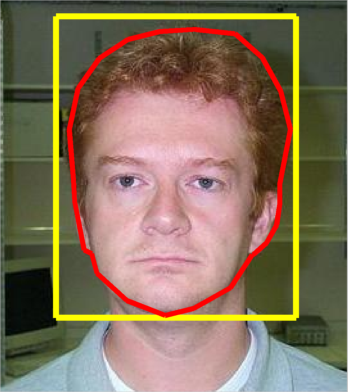
\includegraphics[width=0.25\linewidth]{resources/caltech-101_face_example.png}
  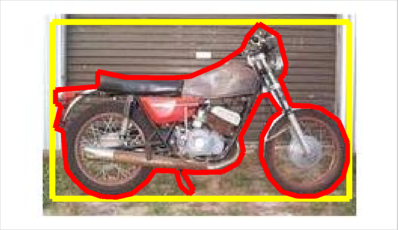
\includegraphics[width=0.4\linewidth]{resources/caltech-101_motorbikes_example.png}
  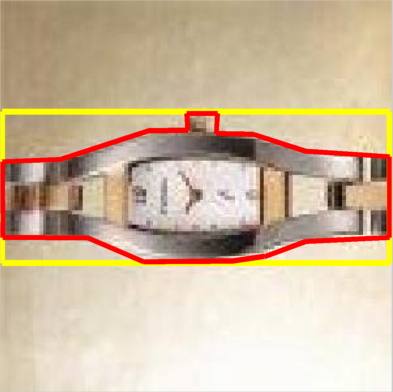
\includegraphics[width=0.25\linewidth]{resources/caltech-101_watch_example.png}\\
  \caption{Caltech-101 examples with annotated ground truth (bounding boxes and the foreground region).}
  \label{fig:caltech}
  \end{center}
\end{figure}
%
The experiments were conducted with the popular Caltech-101~\cite{FeiFerPer:2006} data
set. We preferred Caltech-101 over the more recent data sets, such as
Caltech-256~\cite{Caltech256}, Pascal VOC~\cite{EveGooWil:2010} and
ImageNet~\cite{imagenet}, since they contain substantial 3D view point changes
(e.g. car frontal vs. car side) which are not expected to be solved
on the local feature level.
%For compactness and clarity, the results are reported for the following ten categories which
%represent well the overall performance variation: \textit{watch}, \textit{stop\_sign}, \textit{starfish},
%\textit{revolver}, \textit{euphonium}, \textit{dollar\_bill}, \textit{car\_side},
%\textit{airplanes}, \textit{Motorbikes} and \textit{Faces\_easy}.
The foreground masks available in the data set were used to remove features detected
in the background (Fig.~\ref{fig:caltech}). Affine correspondence between category examples were established
by manually annotating 5-12 landmarks per category and estimating the pair-wise image
transformations using the direct linear transform~\cite{HarZis:2003}. Examples with
annotated landmarks are shown in Fig.~\ref{fig:affine_example1}.
For this experiment we used repeatedly 25 random pairs of images from each category.
% (tot. of 500 images).
%
\begin{figure}[h]
\begin{center}
\subfloat{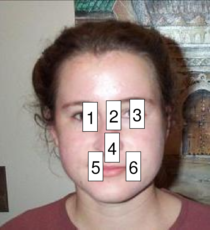
\includegraphics[height=0.2\linewidth]{resources/lm/lm_examples_cat01_img01.png}}
\subfloat{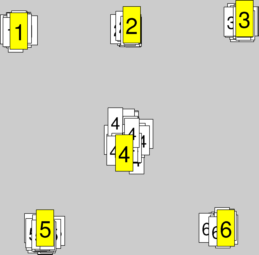
\includegraphics[height=0.2\linewidth]{resources/lm/lm_cat01.png}}~
\subfloat{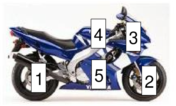
\includegraphics[height=0.2\linewidth]{resources/lm/lm_examples_cat02_img07.png}}
\subfloat{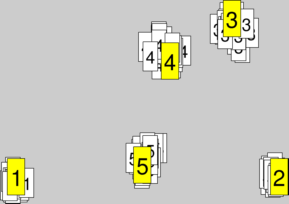
\includegraphics[height=0.2\linewidth]{resources/lm/lm_cat02.png}}\\
%\subfloat{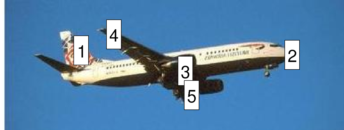
\includegraphics[height=0.1\linewidth]{resources/lm/lm_examples_cat03_img08.png}}
%\subfloat{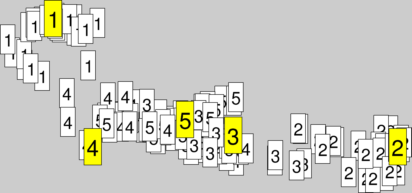
\includegraphics[height=0.1\linewidth]{resources/lm/lm_cat03.png}}~
%\subfloat{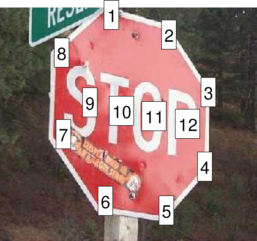
\includegraphics[height=0.16\linewidth]{resources/lm/lm_examples_cat09_img01.png}}
%\subfloat{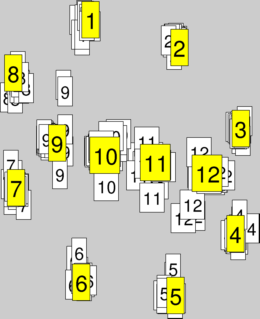
\includegraphics[height=0.16\linewidth]{resources/lm/lm_cat09.png}}\\
%\subfloat{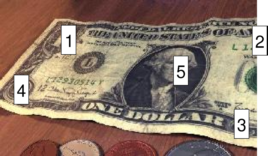
\includegraphics[height=0.12\linewidth]{resources/lm/lm_examples_cat05_img04.png}}
%\subfloat{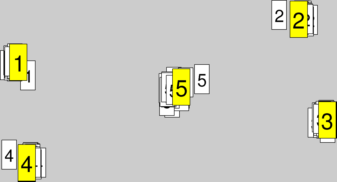
\includegraphics[height=0.12\linewidth]{resources/lm/lm_cat05.png}}~
%\subfloat{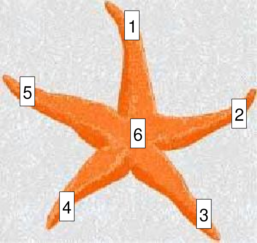
\includegraphics[height=0.14\linewidth]{resources/lm/lm_examples_cat08_img02.png}}
%\subfloat{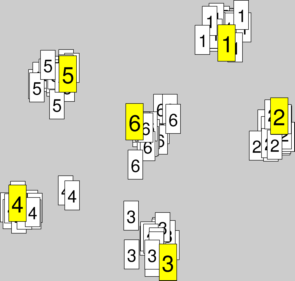
\includegraphics[height=0.14\linewidth]{resources/lm/lm_cat08.png}}\\
%\subfloat{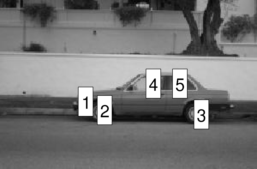
\includegraphics[height=0.14\linewidth]{resources/lm/lm_examples_cat04_img02.png}}
%\subfloat{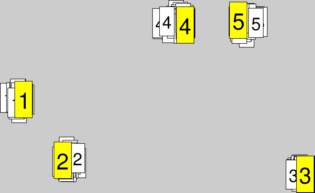
\includegraphics[height=0.14\linewidth]{resources/lm/lm_cat04.png}}~
%\subfloat{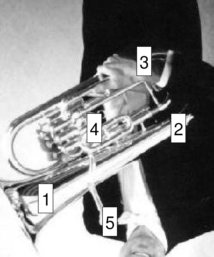
\includegraphics[height=0.14\linewidth]{resources/lm/lm_examples_cat06_img02.png}}
%\subfloat{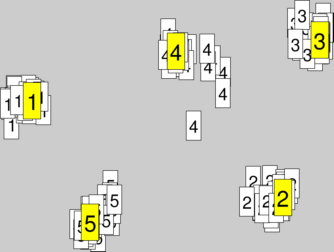
\includegraphics[height=0.14\linewidth]{resources/lm/lm_cat06.png}}\\
\subfloat{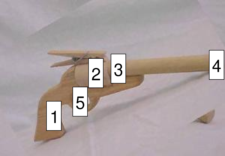
\includegraphics[height=0.17\linewidth]{resources/lm/lm_examples_cat07_img10.png}}
\subfloat{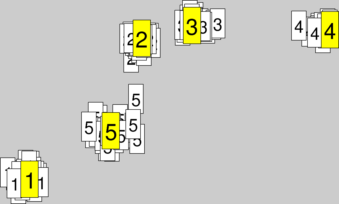
\includegraphics[height=0.17\linewidth]{resources/lm/lm_cat07.png}}~
\subfloat{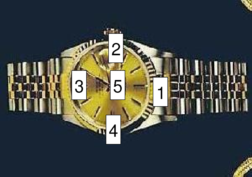
\includegraphics[height=0.17\linewidth]{resources/lm/lm_examples_cat10_img18.png}}
\subfloat{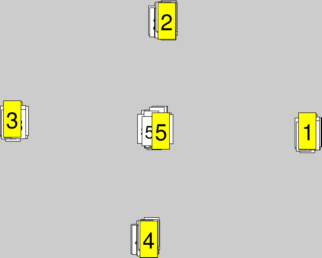
\includegraphics[height=0.17\linewidth]{resources/lm/lm_cat10.png}}
\caption{Object class examples with annotated landmarks (leftmost in each image pair) and 50 examples (affine) projected into
a single space (denoted by the yellow tags). The image diagonal normalised (resolution independent) two standard deviations are
0.0158, 0.0297, 0.0486 and 0.0177, respectively. The part variances imply class specific spatial variance of object parts.}%  {\color{blue} Anders: does the last information on the landmarks tell something about the intra-class variation of the parts, or does this figure simply show the (small) spatial variation of the ``same''  parts for the four example classes?}}
% The two standard deviations of the image diagonal normalised projection errors are (from left to right and top to bottom):
%0.0158,
%0.0297,
%0.1701,
%0.0460,
%0.0304,
%0.0373,
%0.0194,
%0.0641,
%0.0486, and
%0.0177.
\label{fig:affine_example1}
\end{center}
\end{figure}
%

%
\subsection{Region detectors}
%
In our preliminary work we evaluated the following nine
detectors~\cite{LanKanKam:2012}:
\begin{compactenum}
\item Two implementations of the difference of Gaussian: \textit{sift} and \textit{dog-vireo}
\item Harris-Laplace: \textit{harlap-vireo}
\item Laplacian of Gaussian (log): \textit{log-vireo}
\item Three implementations of the Hessian-affine: \textit{hessaff}, \textit{hessaff-alt} and \textit{hesslap-vireo} 
\item Speeded-up robust features: \textit{surf}
\item Maximally stable extramal regions: \textit{mser}
\end{compactenum}
The detectors are publicly available:
 \textit{*-vireo} implementations in Zhao's
Lip-vireo toolkit (\url{http://code.google.com/p/lip-vireo}),
\textit{hessaff} and \textit{hessaff-alt} (by Mikolajczyk) at
\url{http://featurespace.org}, \textit{surf} at the
authors'~\cite{BayEssTuy:2008} web site and \textit{mser} and \textit{sift} in
the popular VLFeat toolbox (\url{http://vlfeat.org}).

The best achieved average repeatability was $33.7\%$ (\textit{dog-vireo}) and the
largest average number of corresponding regions $57.4$ (\textit{hesslap-vireo}). The
best three detectors based on both repeatability and number of regions were
\textit{hesslap-vireo} ($30.6\%$, $57.4$), \textit{hessaff} ($25.3\%$, $47.8$) and
log-vireo ($26.3\%$, $46.5$). For comparison, the hessaff and the VLFeat
SIFT descriptors were also included here.
% and since detector-descriptor combinations using the hessaff
%detector were superior in our preliminary work, we selected hessaff for this
%work as well. In addition, to compare the ``original idea''
%by Lowe~\cite{Low:2004} and state-of-the-art, we also included SIFT detector
%from VLFeat toolbox.

To bring our experiments up-to-date, we tested the recently proposed keypoint
detectors: BRIEF~\cite{brief}, BRISK~\cite{brisk}, ORB~\cite{orb} and
FREAK~\cite{freak}. The best results were obtained with ORB included in
the OpenCV library (\url{http://opencv.org}) and it was
selected in this work (\textit{orb}). Moreover,
dense sampling has replaced detectors in the top methods
(see, e.g., the results of Pascal VOC 2011~\cite{VOC:2011}) and lately
also dense interest points have been proposed~\cite{Tuy:2010}. Therefore
we added the dense SIFT in VLFeat (\url{http://vlfeat.org})
to our evaluation (\textit{dense}).


%
\subsection{Performance measures and evaluation}
%
For the detector performance evaluation, we adopted the test protocol in~\cite{MikTuySch:2005}.
Interest points are first extracted from images. The interest points detected inside the
object area (Caltech-101 foreground) are selected for the evaluation.
%
For each image pair, points from the first image are projected onto the second image by the
affine transformation estimated using the annotated landmarks.
The landmarks projected on a randomly selected example of each category
are demonstrated in Fig.~\ref{fig:affine_example1} with the
two standard deviations corresponding to the 95\% error distributions.
%Only features covered by
%both images are considered, though in this case practically all the features
%fulfill that requirement.
Interest regions are described by 2D ellipses and
a sufficient spatial overlap of two normalised ellipses within the image pair under consideration is accepted as a correct correspondence. We thus have a {\em corresponding region}, or simply a {\em correspondence}.
The number and rate of correspondences for each detector is of interest. A detector performs well
if the total number is large and also reliably if the ratio of correct matches is high.
We used the parameter settings
from~\cite{MikTuySch:2005}: 40\% overlap error threshold and normalisation of the ellipses to
the radius of 30 pixels. %\commentNK{This is a bit unclear for me but experts might now}

The reported performance numbers are the average number of corresponding regions between
image pairs and the repeatability rate, i.e. the ratio between the corresponding 
regions and the total number of detected regions.

\subsection{Results}
%
\begin{figure}[h]
\begin{center}
\subfloat[]{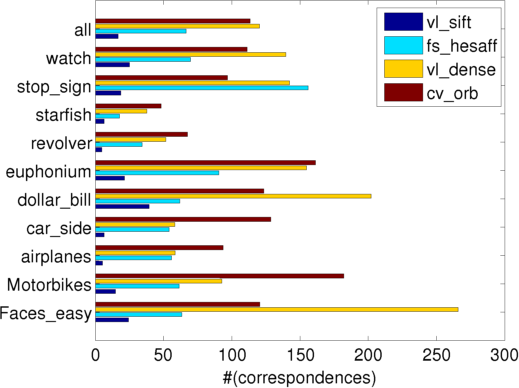
\includegraphics[width=0.8\linewidth]{resources/joni_results/PLOT_detectors_benchmark1report1-detcor-avg.png}}\\
\subfloat[]{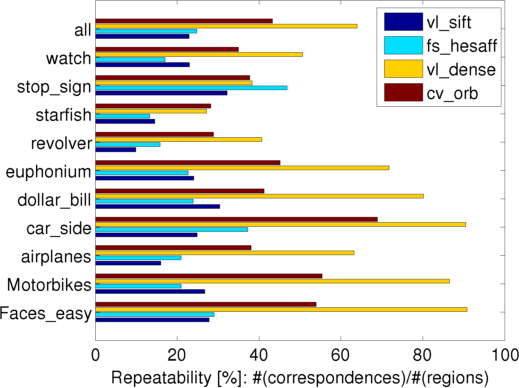
\includegraphics[width=0.8\linewidth]{resources/joni_results/PLOT_detectors_benchmark1report1-detrep-avg.png}}\\
%\subfloat[]{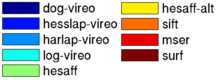
\includegraphics[width=0.3\linewidth]{resources/ville_results/detector-legend.png}}
\subfloat[]{\scriptsize
\begin{tabular}{|l|l|l|}
\hline
\textbf{Detector} & \textbf{Avg \# of corr.} & \textbf{Avg. rep. rate}\\
\hline
%\textit{dog-vireo}     & 16.0 & 33.7\%\\
%\textit{hesslap-vireo} & 57.4 & 30.6\%\\
%\textit{harlap-vireo}  & 34.2 & 20.3\%\\
%\textit{log-vireo}     & 46.5 & 26.3\%\\
%\textit{hesaff}        & 47.8 & 25.3\%\\
%\textit{hesaff-alt}    & 25.0 & 23.4\%\\
%\textit{sift}          & 16.2 & 21.5\%\\
%\textit{mser}          & 11.7 & 13.8\%\\
%\textit{surf}          & 27.9 & 32.0\%\\
\textit{vl\_sift}       &  16.7 & 22.9\%\\
\textit{fs\_hessaff}    &  66.5 & 24.8\%\\
\textit{cv\_orb}        & 113.4 & 43.3\%\\
\textit{vl\_dense}       & 120.4 & 64.0\%\\
\hline
\end{tabular}}
\caption{Benchmarking detectors for visual object class matching:
(a) average number of corresponding regions,
%\textit{dog-vireo}: 16.0;
%\textit{hesslap-vireo}: 57.4;
%\textit{harlap-vireo}: 34.2;
%\textit{log-vireo}: 46.5;
%\textit{hesaff}: 47.8;
%\textit{hesaff-alt}: 25.0;
%\textit{sift}: 16.2;
%\textit{mser}: 11.7;
%\textit{surf}: 27.9;
(b) repeatability rates,
%\textit{dog-vireo}: 33.7\%;
%\textit{hesslap-vireo}: 30.6\%;
%\textit{harlap-vireo}: 20.3\%;
%\textit{log-vireo}: 26.3\%;
%\textit{hesaff}: 25.3\%;
%\textit{hesaff-alt}: 23.4\%;
%\textit{sift}: 21.5\%;
%\textit{mser}: 13.8\%;
%\textit{surf}: 32.0\%;
%(c) colour coding of the detectors, and (d) overall results table.\label{fig:results1}}
and (d) the overall results table.\label{fig:results1}}
\end{center}
\end{figure}
%\begin{figure}[h]
%\begin{center}
%\subfloat[]{\includegraphics[width=0.9\linewidth]{resources/detcor-median.png}}
%\subfloat[]{\includegraphics[width=0.9\linewidth]{resources/detrep-median.png}}
%\caption{(a) median number of corresponding regions, (b) median repeatability rate.\label{fig:results1_median}}
%\end{center}
%\end{figure}
%
The results of the detector experiment are shown in Fig.~\ref{fig:results1}.
The main difference as compared to our preliminary work~\cite{LanKanKam:2012}
is that the best of recently proposed detectors, ORB, and the simple
dense sampling are clearly superior to the earlier winner,
the Hessian-affine detector by Mikolajczyk. The difference to the original detector by Lowe
is almost by order of magnitude better in terms of the number of
correspondences. Clearly, with ORB or dense sampling there
are much more regions to match ($> 100$ on average). Some less favourable
properties of dense sampling are discussed in Sec.~\ref{sec:challenging}.
%\anders{Should we note that the dense matching only performs so well (extremely high repeatability rates), simply because there is a small affine transformation between the 25 sampled image pairs in each category? Otherwise, the reader may think we've found a holy grail. The dense sampling would e.g. not perform so well for Mikolajczyk's benchmark, right?}
%There are significant differences between the different categories.
%Dollar bill and stop sign are generally the easiest, as expected due to
%lower variation in their visual appearance, while the airplanes, car side views and revolvers are
%the most difficult. For the airplanes this
%can be explained by the fact that one of the landmarks is placed on the wing resulting in
%3D pose changes instead of 2D affinities.
%The numbers for all categories are by order of magnitude smaller than for the fixed
%scenes in~\cite{MikTuySch:2005}, being tens of correspondences instead of hundreds of
%them.
%\commentNK{What do we learn from that? Categorization is quite a different problem requiring probably features with higher level of abstraction}


%------------------------------------------------------------------------- 
%
\section{Comparison of Local Region Descriptors\label{sec:descriptorcomparison}}
%
A good region descriptor for the object classification problem should be
discriminative to match only correct regions, and also tolerate
small appearance variation between category examples. These requirements are
general for feature extraction in computer vision and image
processing. The descriptor performances were obtained in the original
work~\cite{MikSch:2005} by computing statistics of the correct and false
matches. In the case of classification, the descriptor matches are expected to
be weaker due to increased variance in the visual appearance of regions.
For example, scooters and road bikes are both in the
Caltech-101 motorbikes category, but their pair-wise similarity
is much weaker than between two scooters or two road bikes.
%Moreover, there is natural variation in the spatial configurations
%of the regions (constellation deformation).
%Therefore, we
%need to tailor the original method to cope with these two sources
%of variation.

%It turns out that there is a strong discrepancy between mean and median
%results and therefore we propose an alternative measure, {\em coverage}, which
%measures the number of images ``covered'' with at least the given number $N$ of correspondences (coverage-$N$). 
%This complements the original evaluation criteria, since we get
%quantitative numbers for how many image pairs at least $N$ 
%correct matches can be found - a few pairs of huge number of matches
%do not distort the results as with the mean number of matches.


%To evaluate the performance of local descriptors selected we simply
%count matches and calculate statistics out of them. Test protocol used in
%\cite{MikSch:2005} is not suitable for this evaluation because the task for
%descriptors is not exactly the same. As we are searching for matches between
%various items in the same object category, the number of matches we can
%assume to be found is significantly lower than if we would try to find
%matches between two images taken at the same scene.

%Although the task of finding matches is not easy, in many cases several 
%matches can be found. If a few matches for an image pair is enough, depends on
%the application. Combining matches of several methods is also a possibility
%that can increase the number of found matches especially when there are
%different kinds of source images in use.

%We use term ``coverage'' to show in how many of the image pairs descriptor
%matches were found. Coverage-n then shows the pairs where $ n $ or more
%matches are found. It can reveal some properties of descriptors as some
%have ability to obtain a few matches even in very challenging image pairs 
%that with most descriptors no matches can be found. It is important to note that
%used detector affects this as it determines the spatial locations in the 
%image that descriptors are calculated for.

%
\subsection{Available descriptors}
%
In our preliminary work we evaluated the following six
combinations~\cite{LanKanKam:2012}:
\begin{compactenum}
\item Hessian-affine and SIFT
\item Hessian-affine and linear filters
\item Alternative (Vireo) implementation of Hessian-affine and SIFT
\item Original SIFT detector and SIFT descriptor
\item Alternative (Vireo) implementation of SIFT and SIFT
\item SURF and SURF
\end{compactenum}
The combinations 1) and 2) utilising Mikolajczyk's implementation
of Hessian-affine detector were clearly superior to other methods.
The Hessian-affine and SIFT achieved the average number of matches
$66.1$ and median $46.0$.

To complete the previous experiments, we here include the
dense sampling and the best of the fast detectors (ORB) and
descriptors (BRIEF). The following combinations will be reported:
{\em fs\_hessaff+fs\_sift} (FeatureSpace implementation),
{\em cv\_orb+cv\_brief} (OpenCV implementation),
{\em cv\_orb+cv\_sift} (OpenCV, to compare SIFT and BRIEF),
{\em vl\_dense+vl\_sift} (VLFeat implementation).

%
\subsection{Performance measures and evaluation\label{sec:descrperformance}}
In the experiments for this article, 
it turned out that the simplified version of Mikolajczyk's descriptor
performance measure proposed in~\cite{LanKanKam:2012} produces overly optimistic
results. Therefore in this work, we revert back to the original measure with an
ellipse overlap threshold and using the nearest neighbour (without the descriptor
matching threshold)~\cite{MikSch:2005}.
%\commentNK{I would take out the first two sentences, since it is an unnecessary detour.} 
%In our previous work in~\cite{LanKanKam:2012}, we replaced the Mikolajczyk's
%matching criterion (the ellipse overlap error used in the detector evaluation),
%with a simpler and less strict ellipse centroid distance threshold. That,
%however, lead to over-optimistic results and therefore for this work
%we adopted the original criterion from~\cite{MikSch:2005}.
At first, descriptors are computed for
all detected regions (foreground only). Images are processed
pair-wise and best matches for each region is selected from
full distance matrices.
It is worth noting
that the rule proposed in~\cite{Low:2004} for discarding ``bad regions''
(ratio between the first and the second best is less than $1.5$) must
not be used with object classes since it would produce virtually no matches
at all. This can be explained by the fact that matches are
never as good as in the wide baseline setting.
We used the maximum ellipse
overlap error $50\%$ from~\cite{MikSch:2005} for finding detector correspondences.
% (note that the detector evaluation
%used the more strict limit of $40\%$). \commentNK{Why?}
%This rule is default in many implementations, but it makes
%the matching performance collapse. %The rule discards outliers in the wide baseline case.
%%: if the distance to the second best match is below
%%Next, due to a large number of false and a small
%%number of correct matches, we adopted the rule proposed 
%%in~\cite{Low:2004}: if the distance to the second best match is below
%%$1.5$ times the distances to the best, the match between these points
%%is removed as incorrect.

%Our spatial verification stage differs from~\cite{MikSch:2005} by
%being less strict since the original rule provides only a few matches for the 
%most pairs. In the original rule, the regions were described by
%ellipses, and for the spatial verification the ellipses were projected onto
%each other using the estimated affine transformation. If a sufficient 
%overlap occurred for the ellipses, then the match was accepted.
%In our case, however, the categories have natural variation in
%their spatial structure. This natural variation
%cannot be exactly encoded into affine transformation and
%therefore the matches are not exact even for the ground truth landmarks as demonstrated in
%Fig.~\ref{fig:affine_example1}. The two standard deviations vary
%between 0.0158 (Faces\_easy) and 0.0641 (euphonium). The airplanes category is an outlier due to the one no%n-2D landmark on the wing tip (0.1701).  However, for ellipse overlap
%computation, even a small difference in the ellipse centroid may have
%an enormous effect to the overlap area~\cite{MikTuySch:2005}. The
%configuration is sufficiently affine over views of a same planar scene, but
%for VOC evaluation we needed to replace the ellipse overlap rule with a distance
%threshold between the ellipse centroids. For resolution independence, the distances were normalised with
%the image diagonal and in our evaluation we discarded
%matches if the distance was greater than $0.05$. This threshold covers the two
%standard deviations of the ground truth landmarks and over 95\% of the landmarks are within 
%this distance.

Our performance numbers are the average number of matches and median
%\commentNK{Wouldn't it make more sense to then use also the median for the detectors?}
number of matches. The median is used to suppress the effect of
several too well matching pairs (same person, identical
stop signs, etc.)
%For applications, it is also important to know how many matches
%are guaranteed to be found, and thus,
%%This can vary between images and is not uniform if the difference between the
%%average and median is large. Thus,
%we also report ``coverage'' numbers (Sec.~\.
%%, i.e. a 
%%number of image pairs for which at least N matches have been found
%%({\em coverage-N}). \anders{I don't think we need to re-explain the coverage term here, so we could remove the ``, i.e...'' part from this sentence.}

%
\subsection{Results\label{sec:results1}}
%
%
\begin{figure}[h]
\begin{center}
\subfloat[]{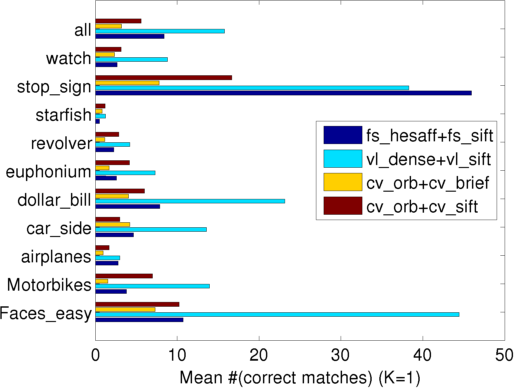
\includegraphics[width=0.8\linewidth]{resources/joni_results/result-figure-report1-mean-all-besmatches-1.png}}\\
\subfloat[]{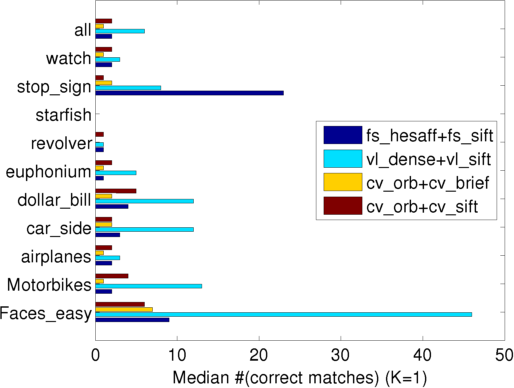
\includegraphics[width=0.8\linewidth]{resources/joni_results/result-figure-report1-median-all-besmatches-1.png}}\\
\subfloat[]{%
\begin{tabular}{|l|l|l|}
\hline
\textbf{Detector+descriptor} & \textbf{Avg \#} & \textbf{Med \#}\\
\hline
\textit{fs\_hessaff+fs\_sift}      &  8.4 & 2\\
\textit{vl\_dense+vl\_sift}        & 15.8 & 6\\
\textit{cv\_orb+cv\_brief}        &  3.2 & 1\\
\textit{cv\_orb+cv\_sift}         &  5.6 & 2\\
\hline
\end{tabular}
} % End subfloat
\caption{Descriptor evaluation: (a) average number of matches per class,
%\textit{sift+sift}: 2.6;
%\textit{hesaff+gloh}: 6.3;
%\textit{surf+surf}: 2.75;
%\textit{hessaff+sift}: 6.3;
%\textit{dog-vireo+sift-vireo}: 2.6;
%\textit{hesslap-vireo+sift-vireo}: 3.4;
(b) median,
%\textit{sift+sift}: 1.0;
%\textit{hesaff+gloh}: 0.0;
%\textit{surf+surf}: 1.0;
%\textit{hessaff+sift}: 0.0;
%\textit{dog-vireo+sift-vireo}: 1.0;
%\textit{hesslap-vireo+sift-vireo}: 0.5;
(c) colour coding of the method names, and
(d) overall results table.}
\label{fig:results2}
\end{center}
\end{figure}
%
%The data for this experiment were the same.
The average and median number of matches for the descriptor evaluation
are shown in Fig.~\ref{fig:results2}.
For many classes, the mean and median numbers are very low and
clearly descriptors sampled on the dense grid are superior for
almost all classes, achieving the average of $15.8$ and median of $6$ matches.
%The
%result is verified by the coverage results in Fig.~\ref{fig:results3}
%where the dense sampling based SIFT finds at least 6 matches
%from 13 our 25 images on average. The next best is the Hessian-affine
%with 7 out of 25.
The only exception is the stop signs category for
which the Hessian-affine outperforms dense sampling.

The best results were obtained for the stop signs, dollar bills and
faces, but the overall performance is poor.
The best discriminative methods could still learn to detect these
categories, but it is difficult to imagine naturally emerging
``common codes'' for other classes except the stop signs, faces and
dollar bills.
It is surprising that the best detectors, Hessian-affine and dense
sampling, were able to provide 66 and 120, repeatable regions on average, but
only roughly $10\%$ of these match in the descriptor space.
The main conclusion of these results is that all descriptors perform
poorly in matching similar regions between class examples.
Fortunately, intra-class matching based on descriptors can be improved,
as we will describe in the following section.

%%
%\begin{figure}
%\begin{center}
%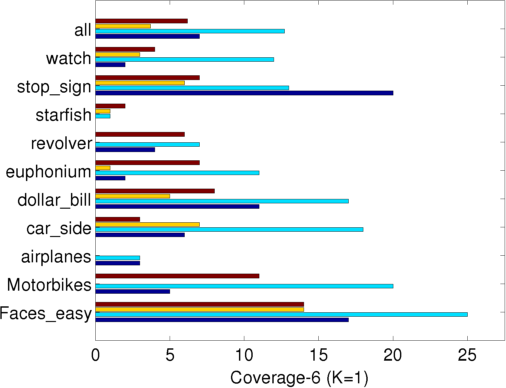
\includegraphics[width=0.8\linewidth]{resources/joni_results/result-figure-report1-coverage-6-besmatches-1.%png}
%\caption{Coverage-6 (number of image pairs for which at least six matching regions found) for the descripto%r evaluation in Fig.~\ref{fig:results2}.}
%\label{fig:results3}
%\end{center}
%\end{figure}


% JONI REMOVED THIS EXPERIMENT SINCE IT DOES NOT REALLY PROVIDE ANYTHING SIGNIFICANT NEW AND
% THE RESULTS ARE EVEN MORE DISAPPOINTING
%\subsection{Validation dataset}
%\joni{Anders: please, repeat the experiment with this data - it should only require
%downloading the data and the new image pair files}\anders{Done! However, I suggest removing the median data since it% is identically zero.}
%One possible explanation for the bad descriptor performance is the poor
%image quality of the most Caltech-101 categories. To study the effect of
%image quality, we collected our own data set, referred to as ``LUTMVPR-12''.
%The data set consist of 12 classes of
%which 6 are the same to Caltech-101 (watches,
%stop signs, revolvers, motorbikes, cars and airplanes). LUTMVPR-12 images
%are of good resolution and quality. The images were collected from Flickr and
%by taking photographs in the town centre. The results are shown
%in Fig.~\ref{fig:results_lut10_1}.
%The results are almost equal to the Caltech-101 results and therefore
%support the previous findings.
%\begin{figure}[h]
%\begin{center} % In both of these figures, X axis is limited to 0-20
%%\subfloat[]{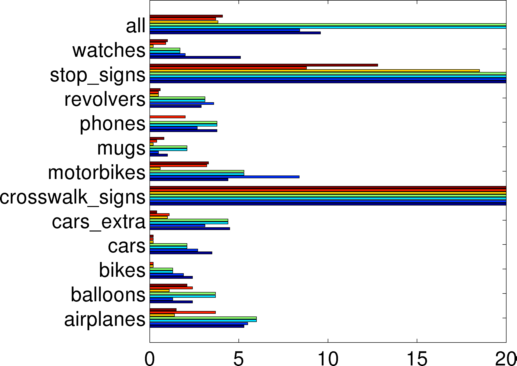
\includegraphics[width=0.44\linewidth]{resources/ville_results/minna-mean-all.png}}
%%\subfloat[]{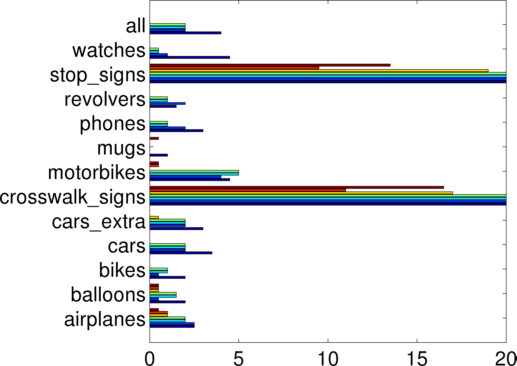
\includegraphics[width=0.44\linewidth]{resources/ville_results/minna-median-all.png}}
%\subfloat[]{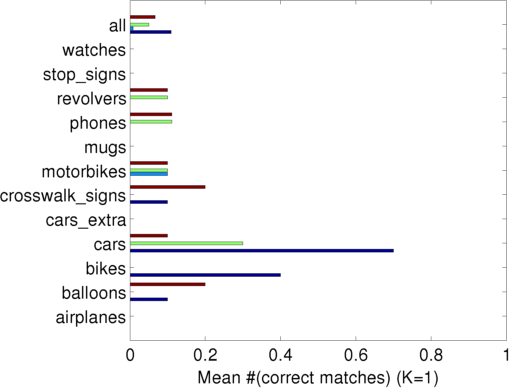
\includegraphics[width=0.44\linewidth]{resources/anders_results/results_minna/mean-all-b1.png}}
%\subfloat[]{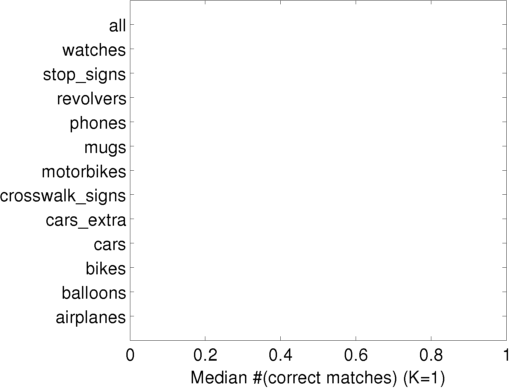
\includegraphics[width=0.44\linewidth]{resources/anders_results/results_minna/median-all-b1.png}}
%%\subfloat[]{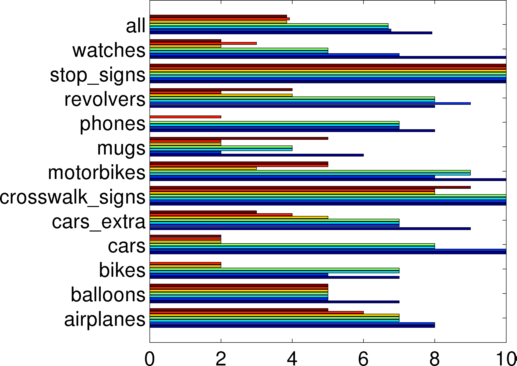
\includegraphics[width=0.44\linewidth]{resources/ville_results/minna-coverage-all.png}}
%\caption{Descriptor evaluation for LUTMVPR-12: (a) average and (b) median
%number of matches per class.
%% (c) coverages for at least one match per class (coverage-1).
%%Coverage number corresponds to the total number of image pairs per class (the maximum is 10).
%\label{fig:results_lut10_1}}
%\end{center}
%\end{figure}
%
%\commentNK{I am a bit unsure about how to present the results. Figure \ref{fig:results_lut10_1} is empty. Also I fee%l - unless it is a standard data base - then more detail on the data (and in particular on the differences to Caltec%h) should be given.}

%
\section{Advanced analysis}
%
In this section, we address the open questions raised during the
detector and descriptors comparisons in Section~\ref{sec:detectorcomparison}
and~\ref{sec:descriptorcomparison}. The important
questions are: why only a few matches are found between different class
examples and what can be done to improve that? Why dense sampling outperforms
all interest point detectors and does it have any drawbacks?

%
\subsection{Beyond single best match}
%
It is obvious that descriptors match better between two images of a same
scene than two different examples of a same object class. However,
it can be assumed that on average two descriptors describing
the same object part should match better than two distant parts.
To test this assumption, every descriptor
can be assigned to multiple best matches. Our next experiment
was motivated by soft assignment, where a single descriptor contributes more
than a single codeword. This approach has been found successful in visual
classification~\cite{AgaTri:2008,TuySch:2007,ChaLemVed:2011}.
In order to measure the effect of multiple assignments, we
establish a new performance measure: \textit{coverage}. Coverage
corresponds to the number of image pairs for which at least N matches
have been found ({\em coverage-N}).
We tested the multiple assignment procedure by accumulating matches over
$n = 1, 2, \ldots, K$ best matches. The corresponding coverages for
$K = 1, 5, 10$ are shown in Fig.~\ref{fig:coverage}. Obviously,
more image pairs contains at least $N=5$ than $N=10$ matches.
With $K=1$ (only the best match) the best method, VLFeat dense SIFT,
finds at least $N=5$ matches in 14 out of
25 image pairs and for $N=10$ 10 matches. When the number of best
matches is increased to $K=5$, the same numbers are 19 and 17, respectively,
showing clear improvement. Beyond $K=5$ the positive effect diminishes, but
it is clearly beneficial to use more than one best match of each
region.
%
\begin{figure*}[htbp]
\begin{center}
\subfloat{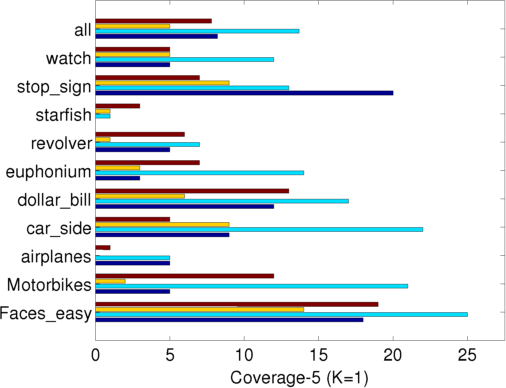
\includegraphics[width=0.32\linewidth]{resources/joni_results/result-figure-report1-coverage-5-besmatches-1.png}}
\subfloat{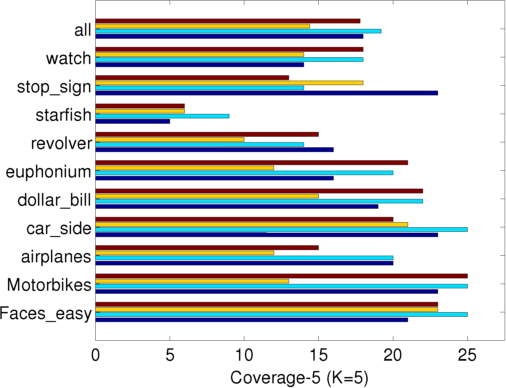
\includegraphics[width=0.32\linewidth]{resources/joni_results/result-figure-report1-coverage-5-besmatches-5.png}}
\subfloat{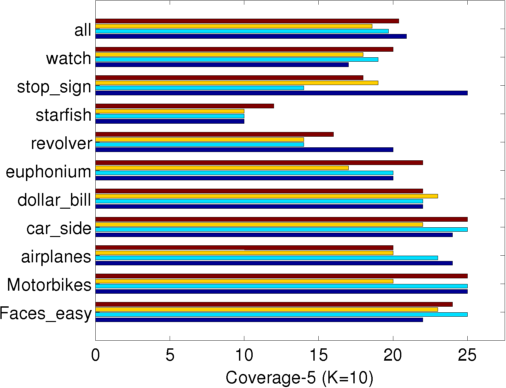
\includegraphics[width=0.32\linewidth]{resources/joni_results/result-figure-report1-coverage-5-besmatches-10.png}}\\
\subfloat{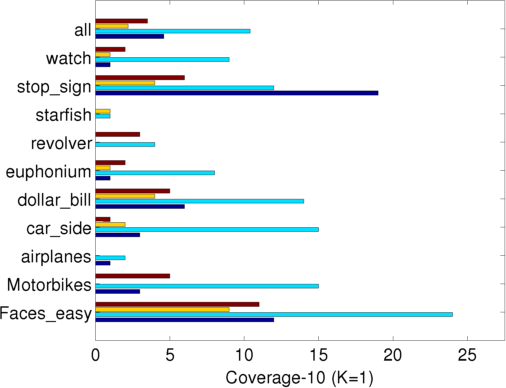
\includegraphics[width=0.32\linewidth]{resources/joni_results/result-figure-report1-coverage-10-besmatches-1.png}}
\subfloat{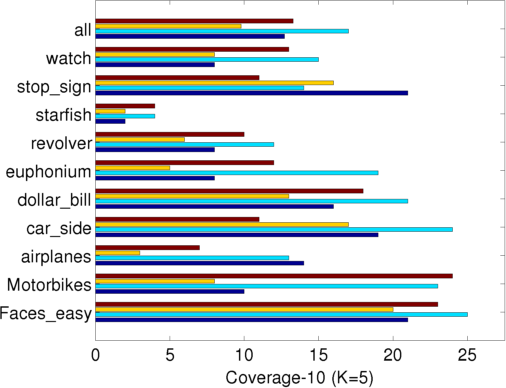
\includegraphics[width=0.32\linewidth]{resources/joni_results/result-figure-report1-coverage-10-besmatches-5.png}}
\subfloat{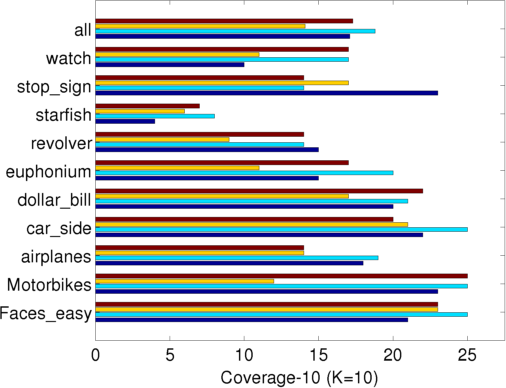
\includegraphics[width=0.32\linewidth]{resources/joni_results/result-figure-report1-coverage-10-besmatches-10.png}}
\caption{Descriptor evaluation results using $K$ best matches. From left to right: $K=1, 5, 10$, respectively. From top down: coverage-5, coverage-10.
\label{fig:coverage}}
\end{center}
\end{figure*}

%
\subsection{Two implementations of the dense {SIFT}}
%
%
\begin{figure}[h]
  \begin{center}
    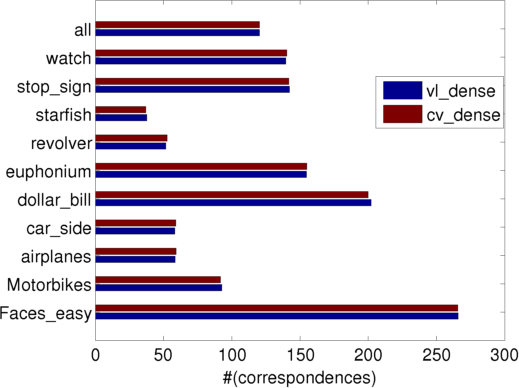
\includegraphics[width=0.48\linewidth]{resources/joni_results/PLOT_detectors_benchmark1report1-detcor-avg_denseonly.png}
    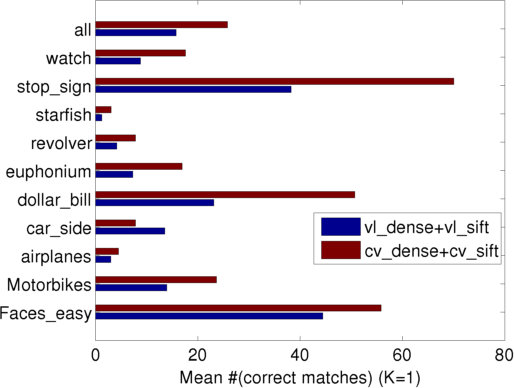
\includegraphics[width=0.48\linewidth]{resources/joni_results/result-figure-report2-mean-all-besmatches-1_denseonly.png}
\caption{OpenCV dense SIFT vs. VLFeat dense SIFT - detector (left) and descriptor (right)
comparison.}
\label{fig:densecomparison}
\end{center}
\end{figure}
%
During the course of work, we noticed that different implementations
of the same method provided different results. Since there are two
popular implementations of dense sampling with the SIFT descriptor,
OpenCV and VLFeat,
we decided to compare the two distinct implementations. The
results corresponding to the previous experiments in 
Sections~\ref{sec:detectorcomparison} and~\ref{sec:descriptorcomparison}
are shown in Fig.~\ref{fig:densecomparison}. %\anders{I would prefer both legends to go ``NorthEast'' in these plots.}
The striking result is
that in the OpenCV implementation the SIFT descriptors match better
than in the VLFeat implementation (OpenCV average 25.8 and median 8 and
for VLFeat 15.8 and 6). For only one class (car side) the VLFeat implementation
is better, but on average OpenCV implementation is better by a clear margin.

%
\subsection{Challenging dense sampling: r-caltech-101\label{sec:challenging}}
%
\begin{figure}[h]
\begin{center}
%  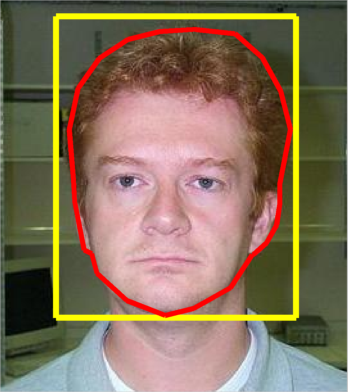
\includegraphics[width=0.25\linewidth]{resources/caltech-101_face_example.png}
%  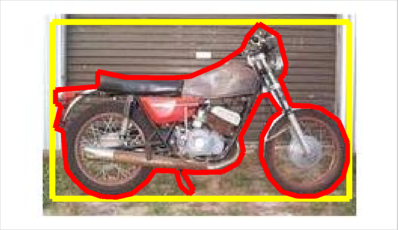
\includegraphics[width=0.4\linewidth]{resources/caltech-101_motorbikes_example.png}
%  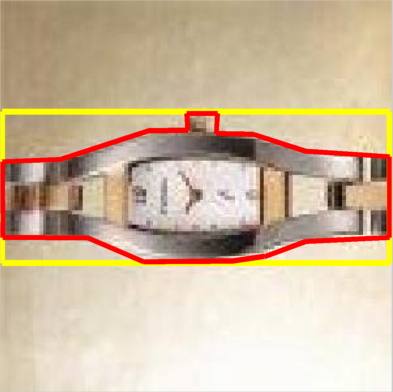
\includegraphics[width=0.25\linewidth]{resources/caltech-101_watch_example.png}\\
  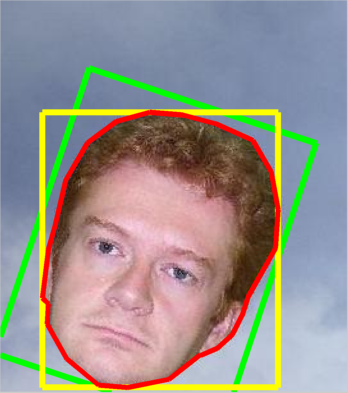
\includegraphics[width=0.25\linewidth]{resources/r-caltech-101_face_example.png}
  \includegraphics[width=0.4\linewidth]{resources/r-caltech-101_motorbikes_example.png}
  \includegraphics[width=0.25\linewidth]{resources/r-caltech-101_watch_example.png}
  \caption{The r-Caltech-101 versions of the original Caltech-101 images in Fig.~\ref{fig:caltech}
    (original bounding box shown by green).\label{fig:rcaltech}}
  \end{center}
\end{figure}
%
%
\begin{figure}
  \begin{center}
    \includegraphics[width=0.48\linewidth]{resources/joni_results/PLOT_detectors_benchmark1report2-rcaltech101-detcor-avg.png}
    \includegraphics[width=0.48\linewidth]{resources/joni_results/result-figure-report2-rcaltech101-mean-all-besmatches-1.png}
\caption{Benchmarks for r-Caltech-101: detector (left) and descriptor (right).
The detector results are almost equivalent to Fig.~\ref{fig:results1}.
In the descriptor benchmark (right, cf. with Fig.~\ref{fig:results2}) the Hessian-affine is almost
unaffected (mean: $8.4~\rightarrow~7.7$) while both dense implementations,
VLFeat ($15.8~\rightarrow~9.7$) and OpenCV ($25.8\rightarrow 16.8$) are severely
affected.}
\label{fig:rcaltechcomparison}
\end{center}
\end{figure}
%
With dense sampling we are concerned with its robustness to changes
in scale and, in particular, orientation, since these are not
estimated similar to interest point detection methods. In this experiment,
we replicated the previous experiments with the two dense sampling
methods and the best interest point detection method using the
randomised version of the Caltech-101 data set, r-Caltech-101~\cite{KinKamLen:2010}.
R-Caltech-101 contains the same objects (foreground), but with varying
random Google backgrounds and the objects have been translated, rotated
and scaled randomly (Fig.~\ref{fig:rcaltech}).

The detector and descriptor results of this experiment are shown in
Fig.~\ref{fig:rcaltechcomparison} %\anders{I would like legends to go ``NorthEast''.}.
Now it is clear that artificial
rotations affect the dense descriptors while Hessian-affine is
almost unaffected. It is noteworthy that the generated pose changes
in r-Caltech-101 are rather small ($[-20^\circ,+20^\circ]$) and
the performance drop could be more dramatic with larger variation.
The obvious research direction would be better scale- and rotation-invariant
dense interest points.

%%
%\subsection{Better descriptors}
%Which descriptor (SIFT vs. BRIEF vs. optimised Gabor).


%------------------------------------------------------------------------- 
%
\section{Discussion}
%
Interest points and regions have been the low-level features in
visual object detection and classification for a decade~\cite{SivZis:2003}.
Recently, supervised low-level features, such as trained
convolution filters in deep neural
networks~\cite{KriSutHin:2012}, have gained momentum, but we
believe that the unsupervised interest point detector-descriptor
approach can be developed further by identifying its weaknesses and
bottlenecks.
In this work, we took a step to this direction by introducing
an evaluation framework of visual
class part detectors and descriptors which provides intuitive
and comparable quantitative results similar to the seminal works
of Mikolajczyk et al.~\cite{MikTuySch:2005,MikSch:2005}.

With the proposed framework we identified the following
important findings:
1) Detectors generally perform well, but descriptors' ability to match
regions over visual class examples collapse.
2) Using multiple, even a few, best matches instead of the single best match
provides significant performance improvement.
3) Dense grid sampling is clearly superior to all interest point detectors.
4) The original SIFT is superior to all recent fast descriptors.
5) Implementation matters, for example, OpenCV SIFT outperforms VLFeat SIFT.
6) Object pose variation severely affects dense sampling
while the best detector (Hessian-affine) is unaffected.

The findings advocate new research on i) better
object descriptors,
ii) dense scale- and rotation-invariant interest point sampling and iii)
alternative matching methods. Some results already exist.
For example, BoW codebook descriptors can be enhanced by merging
descriptors based on co-location and co-activation
clustering~\cite{LeiEttSch:2008}, dense interest points have
been proposed~\cite{Tuy:2010}, and soft-assignment has been shown
to improve BoW codebook matching~\cite{AgaTri:2008}.
Moreover, the success of the standard SIFT in our experiments
justifies further development of better descriptors, not only
faster descriptors. In the new research directions, our evaluation
framework it a useful tool.
%A recent conclusion has been that better descriptors are needed
%for visual object class detection~\cite{RusDenHua:2013,VonKhoMal:2013}
%and our results quantitatively underline this.

% use section* for acknowledgement
\section*{Acknowledgment}


The authors would like to thank...


% Can use something like this to put references on a page
% by themselves when using endfloat and the captionsoff option.
\ifCLASSOPTIONcaptionsoff
  \newpage
\fi



% trigger a \newpage just before the given reference
% number - used to balance the columns on the last page
% adjust value as needed - may need to be readjusted if
% the document is modified later
%\IEEEtriggeratref{8}
% The "triggered" command can be changed if desired:
%\IEEEtriggercmd{\enlargethispage{-5in}}

% references section

% can use a bibliography generated by BibTeX as a .bbl file
% BibTeX documentation can be easily obtained at:
% http://www.ctan.org/tex-archive/biblio/bibtex/contrib/doc/
% The IEEEtran BibTeX style support page is at:
% http://www.michaelshell.org/tex/ieeetran/bibtex/
\bibliographystyle{IEEEtran}
% argument is your BibTeX string definitions and bibliography database(s)
%\bibliography{IEEEabrv,../bib/paper}
\bibliography{intraclass}
% <OR> manually copy in the resultant .bbl file
% set second argument of \begin to the number of references
% (used to reserve space for the reference number labels box)
%\begin{thebibliography}{1}
%
%\bibitem{IEEEhowto:kopka}
%H.~Kopka and P.~W. Daly, \emph{A Guide to \LaTeX}, 3rd~ed.\hskip 1em plus
%  0.5em minus 0.4em\relax Harlow, England: Addison-Wesley, 1999.
%
%\end{thebibliography}

% biography section
% 
% If you have an EPS/PDF photo (graphicx package needed) extra braces are
% needed around the contents of the optional argument to biography to prevent
% the LaTeX parser from getting confused when it sees the complicated
% \includegraphics command within an optional argument. (You could create
% your own custom macro containing the \includegraphics command to make things
% simpler here.)
%\begin{IEEEbiography}[{\includegraphics[width=1in,height=1.25in,clip,keepaspectratio]{mshell}}]{Michael Shell}
% or if you just want to reserve a space for a photo:

\begin{IEEEbiography}{Michael Shell}
Biography text here.
\end{IEEEbiography}

% if you will not have a photo at all:
\begin{IEEEbiographynophoto}{John Doe}
Biography text here.
\end{IEEEbiographynophoto}

% insert where needed to balance the two columns on the last page with
% biographies
%\newpage

\begin{IEEEbiographynophoto}{Jane Doe}
Biography text here.
\end{IEEEbiographynophoto}

% You can push biographies down or up by placing
% a \vfill before or after them. The appropriate
% use of \vfill depends on what kind of text is
% on the last page and whether or not the columns
% are being equalized.

%\vfill

% Can be used to pull up biographies so that the bottom of the last one
% is flush with the other column.
%\enlargethispage{-5in}



% that's all folks
\end{document}


